\chapter{Pr�sentation des entreprises}

\section{Aubay}

\section{Amundi}
Amundi est une filiale du groupe Cr�dit Agricole SA et de la Soci�t� G�n�rale. 
Cette entreprise de gestion des actifs compte parmis les plus grands acteurs de l'industrie de l'asset management
mondial.

Un Asset Manager cr�e et g�re au quotidien des produits de placements, � savoir les OPCVM (Organisme de Placement Commun en Valeurs Mobili�res). Les particuliers et les entreprises souhaitant confier leur argent pour qu'il soit g�r� peuvent faire appel � un Asset Manager. 



\section{Mon stage au sein de l'entreprise}
Dans le cadre de mon projet de fin d'�tude, j'ai int�gr� le service informatique d'Amundi et plus pr�cis�ment l'�quipe MFX, pour Middle Flux, dirrig�e par Jean-Fran�ois Morin.

Le domaine MFX a en charge le d�veloppement et la maintenance des applications utilis�es par le Middle Office Flux Amundi. Celui-ci se d�compose en deux �quipes, la maitrise d'ouvrage (MOA) et la maitrise d'Oeuvre (MOE). Je fais partie de cette derni�re. \\

Dans le domaine on va distinguer quatre types d'applications : 
\begin{enumerate}
	\item Applications permettant d'assurer le cycle de vie des transactions : ETC (Electronic Trade Confirmation) pour le Matching Broker et ETD (Electronic Trade Delivery) pour le r�glement-livraison (le d�positaire et le valorisateur).
	\item Application permettant d'assurer le cycle de vie des titre financiers (Int�gration des op�rations sur titres) : MOCA, Middle Office Corporate Action.
	\item Application permettant l'int�gration des collectes des souscription-rachats sur les fonds Amundi : GSR, Gestion des souscriptions-rachats.
	\item Une plateforme d'�change AMEX dont le p�rim�tre va au del� du domaine MFX, mais dont le d�veloppement et la maintenance du socle technique est de la responsabilit� du domaine MFX. 
\end{enumerate}

Je travaille sur la plateforme Amex et plus pr�cis�ment sur une refonte totale d'un de ses composants, les FlowDetails. Le but principal de cette refonte pour les �quipes utilisant AMEX est une am�lioration des performances.\\ 

\begin{figure}[!h] %on ouvre l'environnement figure
\center
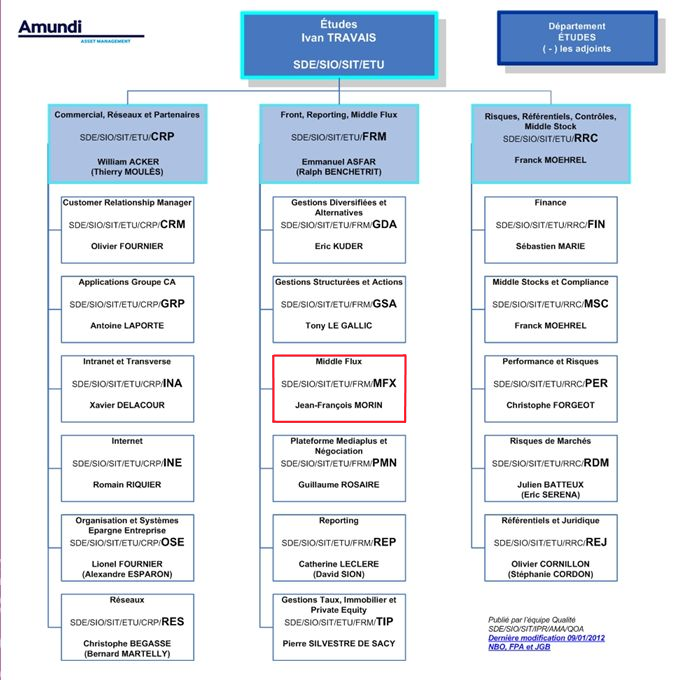
\includegraphics[scale=0.5]{Images/organigrammeEquipes.png}
\caption{Organigramme de Amundi IT Services} %la l�gende
\end{figure} %on ferme l'environnement figure


